\documentclass[11pt]{article}
\usepackage{amsthm, amsmath,textcomp,amssymb,geometry,graphicx,enumerate, mathtools, braket, hyperref, float, listings}
\usepackage[makeroom]{cancel}

\def\Name{Brandon Finley}  % Your name
\def\Homework{2} % Number of Homework
\def\Session{Fall 2020 } % Semester and year
\def\CRS{APPM 5515: High Dimensional Probability}% Course number : course name
\renewcommand\qedsymbol{$\blacksquare$}

\title{\CRS -- \Session --- Homework \Homework} % Course number : course name -- \
\author{\Name}
\markboth{\CRS--\Session\  Homework \Homework\ \Name}{\CRS-- \Session\-- Homework \Homework\ -- \Name}
\pagestyle{myheadings}
\date{}

\textheight=9in
\textwidth=6.5in
\topmargin=-.75in
\oddsidemargin=0.25in
\evensidemargin=0.25in
\setlength\parindent{0pt}
\allowdisplaybreaks

\begin{document}
\maketitle

\begin{enumerate}
	\item Let $x$ and $y$ be indepdent, uniformly distributed random variables on the interval [-1,1]. \\
	Compute 
	\begin{enumerate}
		\item $E[x^2]$
		\item $E[x-y]$
		\item $E[xy]$
		\item $E[(x-y)^2]$
	\end{enumerate}
	\textbf{Solution:} \\ \\
	a) \begin{align*}
		E[x^2] &= \int_{-1}^{1}x^2f_x(x)\,dx \\
		&= \int_{-1}^{1}x^2 \cdot \frac{1}{2}\,dx \\
		&= \frac{1}{6} \cdot 2 \\
		&= \frac{1}{3}
	\end{align*}
	b) \begin{align*}
		E[x-y] &= \int_{-1}^{1}\int_{-1}^{1}(x-y)f_{x,y}(x,y)\,dx\,dy \\
		&= E[x] - E[y] \\
		&= 0 - 0 \\
		&= 0
	\end{align*}
	c) \begin{align*}
		E[xy] &= \int_{-1}^{1}\int_{-1}^{1}xyf_{x,y}(x,y)\,dx\,dy \\
		&= E[x]E[y] \\
		&= 0\cdot0 \\
		&= 0
	\end{align*}
	d) \begin{align*}
		E[(x-y)^2] &= \int_{-1}^{1}\int_{-1}^{1}(x-y)^2f_{x,y}(x,y)\,dx\,dy \\
		&= E[x^2] -2E[xy] + E[y^2] \\
		&= \frac{1}{3} - 2\cdot0 + \frac{1}{3} \\
		&= \frac{2}{3}
	\end{align*}
	\item Let $X = (x_1, x_2, \cdots, x_n)^{T}$ and $Y = (y_1, y_2, \cdots, y_n)^{T}$. $X$ and $Y$ are indepdent, random vectors in $R^n$. 
	\begin{enumerate}
		\item Compute the expected squared distance between $X$ and $Y$, that is $E[||X-Y||^2]$. \\
		\item Computed the expected angle between $X$ and $Y$, that is $E[\angle X, Y]$.
	\end{enumerate}
	\textbf{Solution:} \\\\
	a) Let $Z = X-Y$. Then $Z = (x_1 - y_1, x_2 - y_2, \cdots, x_n - y_n)^T$. This implies that $||X-Y||^2 = ||Z||^2$. Using the properties of a norm, we know this to be $(x_1 - y_1)^2 + (x_2 - y_2)^2 + \cdots + (x_n - y_n)^2$, or more succintly, $\sum_{i = 1}^n(x_i - y_i)^2$.
	We can then plug this into our expectation value to find what we are looking for
	\begin{align*}
		E[||X-Y||^2] &= E[||Z||^2] \\
		&= E[\sum_{i = 1}^n(x_i - y_i)^2] \\
		&= \sum_{i = 1}^nE[(x_i - y_i)^2] \\
		&= \sum_{i = 1}^n \frac{2}{3} \\
		&= \frac{2n}{3}
	\end{align*}
	b) Let us define the L-2 inner product. Then, we know $\langle X,Y \rangle = X \cdot Y = x_1y_1 +x_2y_2 + \cdots + x_ny_n$. Now using the expectation value as a linear operator, we get $E[X \cdot Y] = E[x_1y_1 +x_2y_2 + \cdots + x_ny_n]$. Recall from above that $E[x_iy_i]~\forall i \in N$ is 0. 
	Then we know that $E[X\cdot Y] = 0$. Since the inner product between these two random variables is defined to be zero, then we know \textit{orthogonality} must exist. As such, the angle between the two random variables must be $90^\circ$ or $\frac{\pi}{2}$ radians.

	\item Use Hoeffding inequality to show that
	\begin{equation}
		P\left( \left| \langle x, u \rangle \right| > \epsilon \right) \le 2e^{-2\epsilon^2}
	\end{equation}
	on the interval [-0.5, 0.5]. \\\\
	\textbf{Solution:} \\
	Recall that Hoeffding's inequality states that
	\begin{equation*}
		P \left( \left| S_n - E[S_n] \right| > t \right) \le 2e^{\frac{-2t^2}{\sum_{i=1}^{n}(b_i - a_i)^2}}
	\end{equation*}
	Now back to the problem, we see $\langle x, \textbf{u} \rangle$ is in the place of the absolute value terms. Writing this out we get
	\begin{align*}
		\langle x, u \rangle &=  \langle x,
			\begin{bmatrix}
			\frac{1}{\sqrt{n}},
			\frac{1}{\sqrt{n}},
			\cdots,
			\frac{1}{\sqrt{n}}
		\end{bmatrix}^T \rangle \\
		&= \sum_{i=1}^{n} \frac{1}{\sqrt{n}}x_i \\
		&= \frac{1}{\sqrt{n}}\sum_{i=1}^{n} x_i \\
		&= \frac{1}{\sqrt{n}} S_n
	\end{align*}
	Also note that $E[S_n] = E[\sum_{i=1}^n x_i] = \sum_{i=1}^n E[x_i] = n \cdot 0 = 0$. Now let $t=\epsilon \cdot \sqrt{n}$. 
	Then using Hoeffding's inequality, we can say
	\begin{align*}
		P \left( \left| S_n - E[S_n] \right| > t \right) &= P \left( \left| S_n \right| > \epsilon \cdot \sqrt{n} \right) \\
		&\le 2e^{\frac{-2n\epsilon^2}{\sum_{i=1}^{n}(b_i - a_i)^2}}
	\end{align*}
	Now note that $b_i = 0.5$ and $a_i = -0.5$. Thus, 
	\begin{align*}
		2e^{\frac{-2n\epsilon^2}{\sum_{i=1}^{n}(b_i - a_i)^2}} &= 2e^{\frac{-2n\epsilon^2}{n}} \\
		&= 2e^{-2\epsilon^2}
	\end{align*}
	\item Take $\epsilon = \sqrt{\log20/2} \approx 1.2$ to conclude that the points in $K_n$ concentrate in the thin slab, of thickness $\epsilon$, centered around the hyperplane $\textbf{u}_\perp$. \\\\
	\textbf{Solution:} \\
	Here, we use Hoeffding's inequality to explain why this is the case. In question 3, we calculated the probability of the projection of $x$ onto \textbf{u} is greater than some $\epsilon$.
	Doing this, we found that probability is an incredibly tight bound that gets tight exponentionally. The significiance behind this is that if the probability of the projection of $x$ onto the diagonal vector of the cube outside a given $\epsilon$ is extremely small, then it must be incredibly near to the vector. 
	Thus, we see that the points concentrate onto the thin slab of thickness $\epsilon$.
	
	\item Randomly generate 400 points inside $K_{100}$ and plot the histogram of the distances
	between points and the angle between the vectors from the origin to the points, for
	all pairs of points. Explain your findings in terms of the theoretical analysis that you
	performed in question 2. \\\\
	\textbf{Solution:} \\
	Here we will show how we can use the theory done in question 2 in real applications or simulations. Running the simulation the question gives us, with 400 points inside $K_{100}$ on the interval [-0.5, 0.5], we get the following histograms
	for the expected distance and angle between any two points.
	\begin{figure}[H]
		\centering
		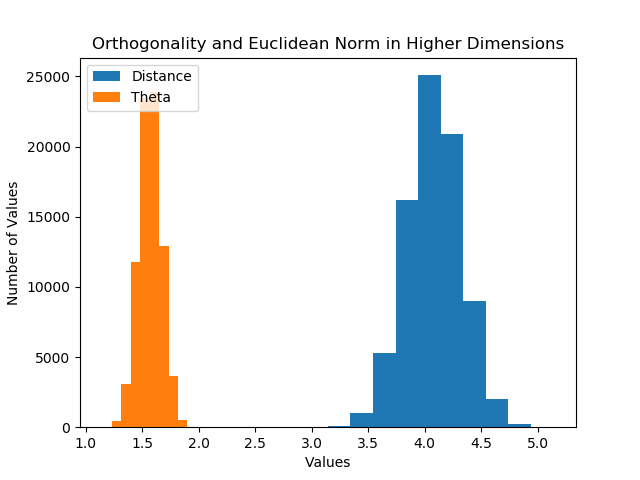
\includegraphics[width = 0.6 \linewidth]{DistanceAngles.png}
		\caption{Histogram of Distance and Angle}
		\label{fig:Hists}
	\end{figure}
	We can see that the expected angle is 1.5 radians, which when plugged into cosine equals zero. This makes sense as it illustrates that in this dimensional space, most points are orthogonal. Moving onto the expected distance, we can apply the same procedure we used in question 2 but on the interval [-0.5, 0.5].
	Doing this, we get $E[x^2] = \frac{1}{12}$. Thus, $E[(x_i - y_i)^2] = \frac{1}{6}$. This then implies that the expected squared distance is $n\cdot\frac{1}{6}$, or that the expected distance is $\sqrt{\frac{n}{6}}$. 
	Finally, pluggin in $n=100$, we get the value to be $\approx 4.0743$. This is consistent with the experiment done. Yay for math!
	\item Derive an expression for the volume V(Q) of 
	\begin{equation}
		Q = [-1, 1] \times \cdots \times [-1, 1]
	\end{equation}
	\textbf{Solution:} \\
	We know the volume of a cube is the product of the length of its sides. Now, for 3 dimensions, that is $l^3$, for 4 dimensions, $l^4$, and so on. This impiles that for an n-dimensional cube, the volume is $l^n$.
	From the cube given above, we see that the side length, $l$, is 1 - (-1) = 2. \\
	Thus,
	\begin{equation*}
		\boxed{V(Q) = 2^n}
	\end{equation*}
	\item Prove that
	\begin{equation}
		\frac{V(B^n(1))}{V(Q)} \to \frac{1}{\sqrt{n}^n} \text{   as n   } \to \infty
	\end{equation}
	\textbf{Solution:} \\
	Given from the problem statement, we know the following
	\begin{equation*}
		V(B^n(1)) = \frac{(\sqrt{\pi})^n}{\Gamma(n/2 + 1)}
	\end{equation*}
	and
	\begin{equation*}
		V(Q) = 2^n
	\end{equation*}
	We also know by Stirling's formula that as $n \to \infty$ we have the following:
	\begin{equation*}
		\Gamma(z+1) \sim \sqrt{2\pi z}\left( \frac{z}{e}\right)^z
	\end{equation*}
	Therefore combing all equations as $n \to \infty$, and setting $z = n/2$, we can arrive at our conclusion.
	\begin{align*}
		\frac{V(B^n(1))}{V(Q)} &= \frac{\left( \sqrt{\pi} \right)^n}{2^n \Gamma(n/2 + 1)} \\
		&\sim \frac{\left(\sqrt{\pi}\right)^n}{2^n \sqrt{\pi n}\left( \frac{n}{2e}\right)^{n/2}} \\
		&= \frac{1}{2^n\sqrt{\pi n}}\left[\sqrt{\frac{2 \pi e}{n}}\right]^n \\
		&\le \frac{1}{(2\sqrt{n})^n} \\
		&\le \frac{1}{\sqrt{n}^n} \\
		&\to 0 \text{ as } n \to \infty
	\end{align*}
	\item Generate 10,000 samples distributed uniformly in $[-1,1]^n$ with algorithm 1, for $n = 1, \cdots, 400$. Plot as a function of $n$. Comment. \\\\
	\textbf{Solution:} \\
	As you can see from the figure below, as $n$ approaches higher dimensions, the number of rejected points dramatically increases. 
	Specifically, it seems to converge to all points being rejected around dimension 25.
	\begin{figure}[H]
		\centering
		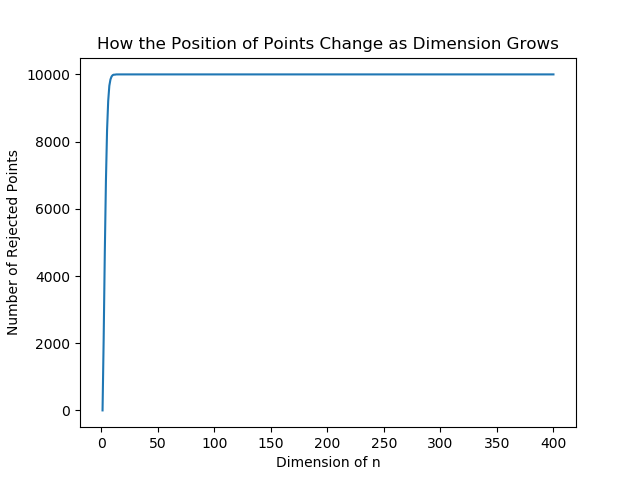
\includegraphics[width = 0.6 \linewidth]{SampledPointsSphere.png}
		\caption{Simulation of Rejected Points Outside Ball}
		\label{fig:RejectPoints}
	\end{figure}
	Looking at question 7 explains why this is the case. In question 7, we calculated the ratio of the volume to the ball compared to that of the cube. 
	As we see, it quickly went to zero. This corroborates our simulation as many of the points inside the cube lied outside the unit ball, meaning that most of the points lied on the surface of the ball.
	This is an interesting finding that I am sure we will cover more of in future lectures.
\end{enumerate}
\begin{center}
	\boxed{{\textbf{| END |}}}
\end{center}
\section*{Appendix}
\lstinputlisting[language=Python]{problem5.py}
\lstinputlisting[language=Python]{problem8.py}
\end{document}